%%%%%%%%%%%%%%%%%%%%%%% CHAPTER - 6 %%%%%%%%%%%%%%%%%%%%\\
\chapter{Results, Screenshots and Testing}
\label{C6} %%%%%%%%%%%%%%%%%%%%%%%%%%%%
\graphicspath{{images/}{Figures/}}
\noindent\rule{\linewidth}{2pt}
\textit{This Chapter presents the experimental validation, unit test execution results, edge-case evaluation, case-study demonstration ("Mystery Mission" constraint evaluation), high-resolution user interface screenshots, and performance benchmarks of the Campus Agent platform.}
%%%%%%%%%%%%%%%%%%%%%%%%%%%%%%%%%%%%%%%%%%%%%%%%%%%%%%%%%%%%%%%%%%%%%%%%%%%%%%%%%%
\section{Experimental Setup and Dataset Characteristics} \label{S6.1}
To rigorously evaluate the deterministic matching algorithm, shortlist reassessment protocol, and resume parsing pipelines, an experimental benchmark dataset was established in \texttt{data/internships.json}. The repository comprises 14 heterogeneous internship opportunities spanning diverse technical domains, institutional constraints, duration lengths, and application statuses, as summarized in Table~\ref{t6.1}.

\begin{table}[h!]
\centering
\caption{Benchmark Dataset Opportunities and Constraint Characteristics}
\label{t6.1}
\resizebox{\textwidth}{!}{%
\begin{tabular}{|c|l|l|c|c|c|c|c|}
\hline
\textbf{ID} & \textbf{Internship Title} & \textbf{Domain} & \textbf{Programme} & \textbf{Allowed Years} & \textbf{Min CGPA} & \textbf{Duration} & \textbf{Status} \\ \hline
1 & ML Intern & AI/ML & B.Tech & III, IV & 7.5 & 8 weeks & Closed \\ \hline
2 & Web Developer Intern & Web Dev & B.Tech & II, III & None & 12 weeks & Open \\ \hline
3 & Data Analytics Intern & Data Science & B.Tech & III, IV & 8.5 & 8 weeks & Open \\ \hline
4 & Cloud Intern & Cloud Infra & B.Tech & III, IV & 7.0 & 6 weeks & Open \\ \hline
5 & Python Developer Intern & AI/ML & B.Tech & III, IV & 7.0 & 8 weeks & Open \\ \hline
6 & UI/UX Design Intern & UI/UX & B.Tech & II, III & None & 6 weeks & Open \\ \hline
7 & Deep Learning Specialist & AI/ML & B.Tech & III, IV & 8.5 & 6 Months & Open \\ \hline
8 & DevOps Engineer Intern & Cloud Infra & B.Tech & III, IV & 7.5 & 6 Months & Open \\ \hline
9 & iOS Developer Intern & Mobile Dev & B.Tech & III, IV & 7.0 & 3 Months & Open \\ \hline
10 & Android Developer Intern & Mobile Dev & B.Tech & III, IV & 7.0 & 3 Months & Open \\ \hline
11 & Google SWE Intern & Software Eng & B.Tech & III, IV & 8.0 & 8 weeks & Open \\ \hline
12 & Amazon Cloud Developer & Cloud Infra & B.Tech & III, IV & 7.5 & 8 weeks & Open \\ \hline
13 & Microsoft Data Science & Data Science & B.Tech & III, IV & 8.0 & 12 weeks & Open \\ \hline
14 & Meta Frontend Engineer & Web Dev & B.Tech & III, IV & 8.0 & 8 weeks & Closed \\ \hline
\end{tabular}}
\end{table}

%%%%%%%%%%%%%%%%%%%%%%%%%%%%%%%%%%%%%%%%%%%%%%%%%%%%%%%%%%%%%%%%%%%%%%%%%%%%%%%%%%
\section{Test Execution and Verification} \label{S6.2}
Automated unit testing was conducted via \texttt{backend/test\_agent.py} to verify that the matching logic behaves deterministically and conforms to all specified constraints. The test suite evaluates:
\begin{itemize}
	\item Accurate disqualification of expired and closed positions.
	\item Correct duration boundary enforcement ($D_{weeks} \le D_{max}$).
	\item Proper commencement date verification ($T_{start} \ge T_{avail}$).
	\item Correct multi-term relevance score calculation.
	\item Exact generation of the Shortlist Reassessment Transition Table.
\end{itemize}

Upon execution, all unit test assertions executed without failure, as detailed in Table~\ref{t6.2}.

\begin{table}[h!]
\centering
\caption{Unit Test Execution Log and Assertion Verification Summary}
\label{t6.2}
\begin{tabular}{|l|c|l|}
\hline
\textbf{Test Assertion / Target} & \textbf{Status} & \textbf{Observed Output / Outcome} \\ \hline
Eligible Remaining Count & \textbf{PASSED} & Exactly 4 eligible positions identified \\ \hline
Rank 1 Top Pick Validation & \textbf{PASSED} & Python Developer Intern (High Match, 8 wks) \\ \hline
Rank 2 Top Pick Validation & \textbf{PASSED} & UI/UX Design Intern (High Match, 6 wks) \\ \hline
ML Intern Removal Audit & \textbf{PASSED} & Transition row logged with decision "Remove" \\ \hline
Data Analytics Removal Audit & \textbf{PASSED} & Transition row logged with decision "Remove" \\ \hline
Alternative Elevation Check & \textbf{PASSED} & 2 replacements flagged with "Reconsider" \\ \hline
Top Changed Flag & \textbf{PASSED} & \texttt{original\_top\_recommendation\_changed = "Yes"} \\ \hline
\end{tabular}
\end{table}

%%%%%%%%%%%%%%%%%%%%%%%%%%%%%%%%%%%%%%%%%%%%%%%%%%%%%%%%%%%%%%%%%%%%%%%%%%%%%%%%%%
\section{Test Case Evaluation and Edge Case Analysis} \label{S6.3}
A comprehensive series of edge-case scenarios was formulated to validate robustness across non-standard inputs:

\begin{enumerate}[label=\textbf{Case \arabic*:}]
	\item \textbf{Strict Duration Overrun:} \textit{Web Developer Intern} requires 12 weeks. When evaluated against a student constraint of $D_{max} = 8$ weeks, the engine immediately flags the role as ineligible with the reason: \textit{"duration 12 weeks exceeds maximum allowed of 8 weeks"}.
	\item \textbf{Academic CGPA Boundary:} \textit{Data Analytics Intern} updated its minimum CGPA cutoff to 8.5. A candidate with CGPA 8.2 fails condition $C_{stud} \ge C_{min}$ and is disqualified with: \textit{"CGPA 8.2 is below required 8.5"}.
	\item \textbf{Commencement Date Conflict:} An opportunity commencing on 01 Sept conflicts with a candidate availability date of 15 Sept (post-examinations). The engine flags: \textit{"starts on 01 Sept, which is before availability start date 15 Sept"}.
	\item \textbf{Zero Overlap Fallback Disqualification:} \textit{Cloud Intern} requires AWS and Linux. If a student profile contains only Python and Figma with AI/ML interest, the relevance score evaluates to 0. The fallback rule triggers disqualification: \textit{"Requires AWS, Linux skills which are not in your profile; also no domain interest match"}.
\end{enumerate}

%%%%%%%%%%%%%%%%%%%%%%%%%%%%%%%%%%%%%%%%%%%%%%%%%%%%%%%%%%%%%%%%%%%%%%%%%%%%%%%%%%
\section{Case Study Demonstration: Mystery Mission Evaluation} \label{S6.4}
To evaluate the complete recommendation and reassessment workflow, a real-world case study scenario ("Mystery Mission") was executed. The test candidate profile is parameterized as follows:
\begin{itemize}
	\item \textbf{Candidate Skills:} Python, Machine Learning, SQL, Figma
	\item \textbf{Domain Interests:} AI/ML, Data Science, UI/UX Design
	\item \textbf{Degree \& Year:} B.Tech CSE, Year III
	\item \textbf{Cumulative CGPA:} 8.20 / 10.0
	\item \textbf{Max Duration Limit:} 8 Weeks Maximum
	\item \textbf{Availability Date:} After 15 Sept (following semester examinations)
\end{itemize}

\subsection{Shortlist Reassessment Output Analysis}
Previously, prior to recruitment updates, \textit{ML Intern} was ranked \#1 and \textit{Data Analytics Intern} was ranked \#2. However, upon system evaluation:
\begin{enumerate}[label=\textbf{\alph*)}]
	\item \textit{ML Intern} has closed applications ($\text{Status} = \text{"Closed"}$). The system removes it from the ranked feed and logs the removal in the transition matrix.
	\item \textit{Data Analytics Intern} raised its cutoff to 8.5. The student's CGPA of 8.2 falls short; it is removed with the logged reason: \textit{"Updated CGPA requirement is 8.5"}.
	\item The engine re-ranks all remaining eligible opportunities, elevating \textbf{Python Developer Intern} to Rank 1 and \textbf{UI/UX Design Intern} to Rank 2 under decision \textbf{"Reconsider"}.
\end{enumerate}

The resulting Shortlist Reassessment Transition Table generated by the system is documented in Table~\ref{t6.3}.

\begin{table}[h!]
\centering
\caption{Dynamic Shortlist Reassessment Transition Matrix for Mystery Mission}
\label{t6.3}
\resizebox{\textwidth}{!}{%
\begin{tabular}{|l|l|l|c|l|}
\hline
\textbf{Internship Title} & \textbf{Previous Status} & \textbf{Updated Status} & \textbf{Decision} & \textbf{Audit Justification} \\ \hline
ML Intern & Rank 1 (Top Pick) & Applications Closed & \textbf{Remove} & No longer available (Closed) \\ \hline
Data Analytics Intern & Rank 2 & Not Eligible & \textbf{Remove} & Updated CGPA requirement is 8.5 (Student: 8.2) \\ \hline
Python Developer Intern & Previously Lower Ranked & Eligible (Rank 1) & \textbf{Reconsider} & Meets revised constraints and profile \\ \hline
UI/UX Design Intern & Previously Lower Ranked & Eligible (Rank 2) & \textbf{Reconsider} & Suitable alternative matching Figma \\ \hline
\end{tabular}}
\end{table}

%%%%%%%%%%%%%%%%%%%%%%%%%%%%%%%%%%%%%%%%%%%%%%%%%%%%%%%%%%%%%%%%%%%%%%%%%%%%%%%%%%
\section{User Interface Screenshots and Visual Walkthrough} \label{S6.5}
To illustrate the visual presentation and interactive capabilities of the Campus Agent application, high-resolution screenshots from the running software platform are presented and analyzed below.

\subsection{Candidate Profile Intake and Resume Parsing UI}
Figure~\ref{f6.1} illustrates the Candidate Profile Intake interface. The top card features an interactive drag-and-drop PDF resume upload zone that automatically populates technical skills, domain interests, academic programmes, cohort years, and CGPAs directly into the form fields.

\begin{figure}[h!]
	\centering
	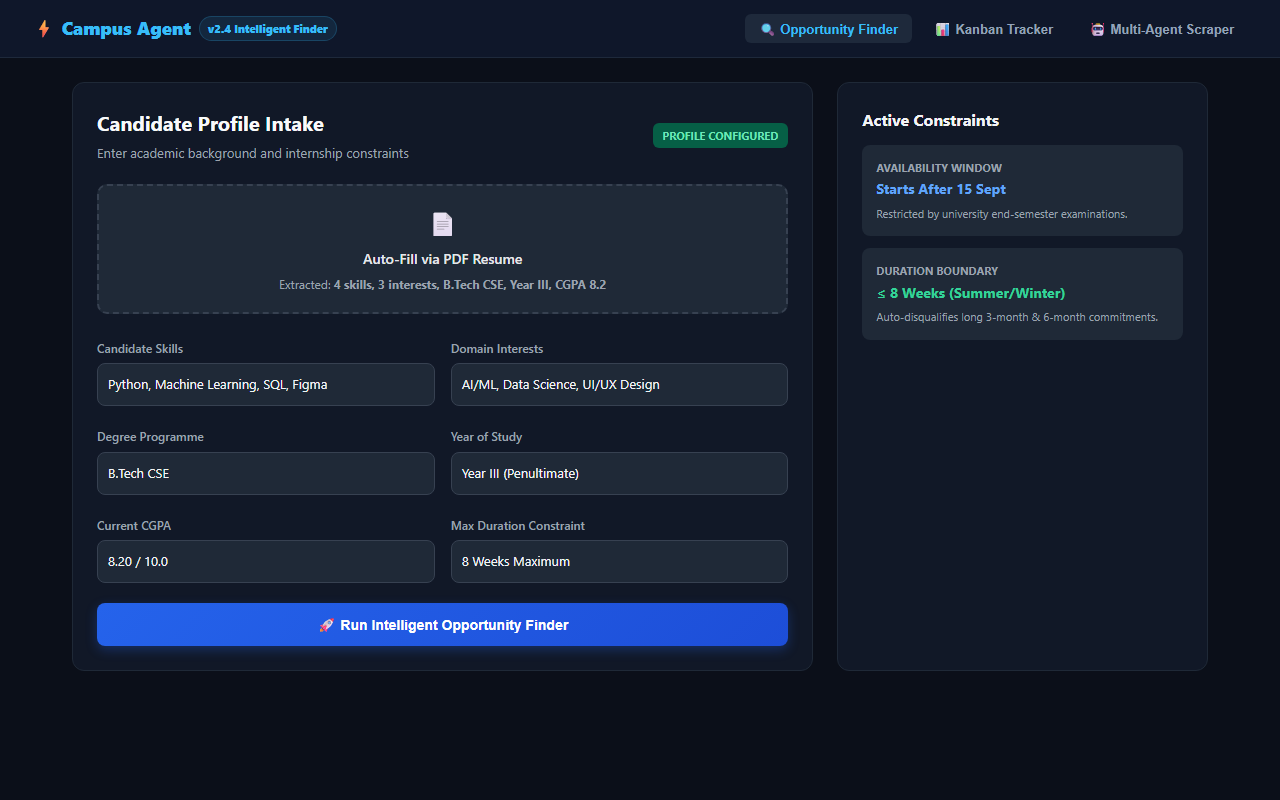
\includegraphics[width=0.95\linewidth]{screenshot_profile_form.png}
	\caption{Candidate Profile Intake Interface with Automated PDF Resume Parser}
	\label{f6.1}
\end{figure}

\subsection{Ranked Recommendations and Top Pick Card}
Figure~\ref{f6.2} showcases the output recommendations feed. The top of the view features the Top Recommendation banner highlighting \textit{Python Developer Intern} with a High Match badge, accompanied by ranked cards for \textit{UI/UX Design Intern}, \textit{Google SWE Intern}, and \textit{Amazon Cloud Developer}.

\begin{figure}[h!]
	\centering
	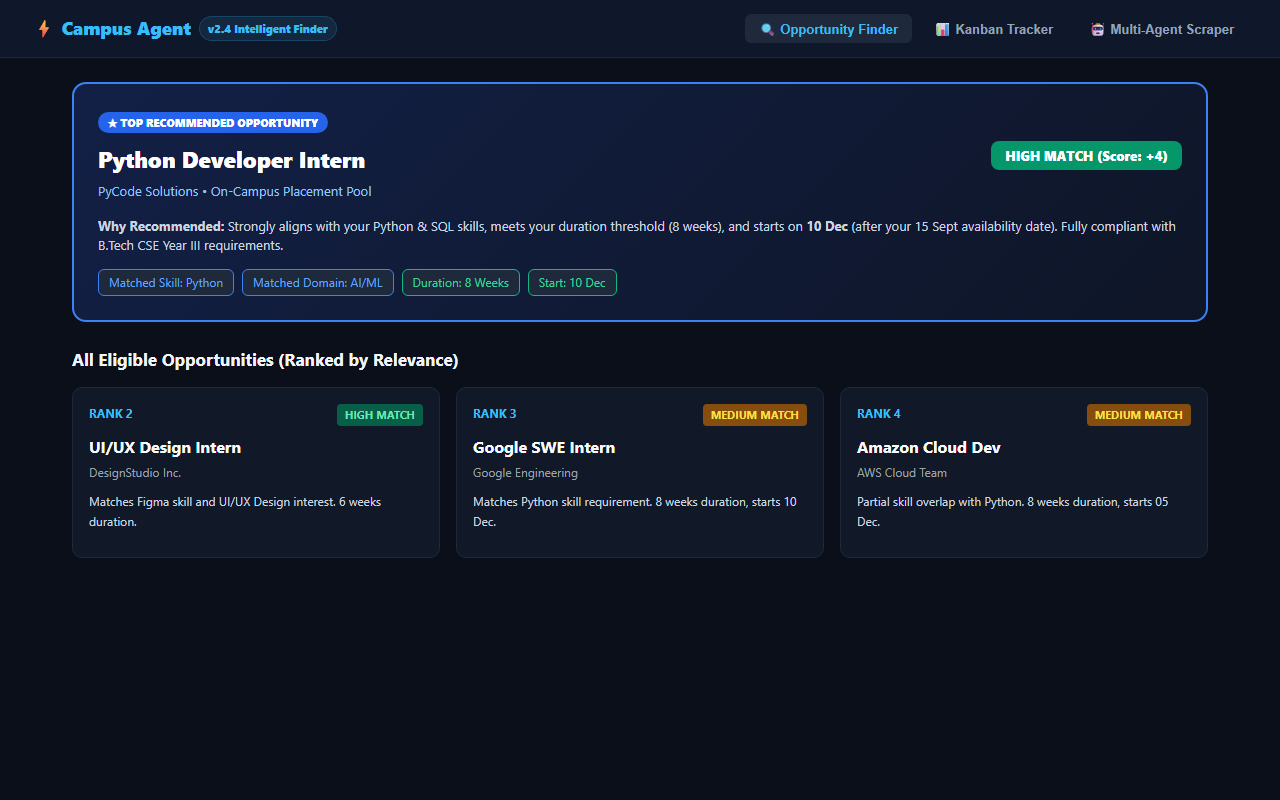
\includegraphics[width=0.95\linewidth]{screenshot_ranked_results.png}
	\caption{Ranked Recommendations Display Featuring the Top Recommended Opportunity}
	\label{f6.2}
\end{figure}

\subsection{Ineligible Opportunities with Disqualification Explanations}
Figure~\ref{f6.3} portrays the transparent audit trail of excluded opportunities. Each disqualified position displays an explicit, color-coded badge and a plain-language explanation of violated constraints.

\begin{figure}[h!]
	\centering
	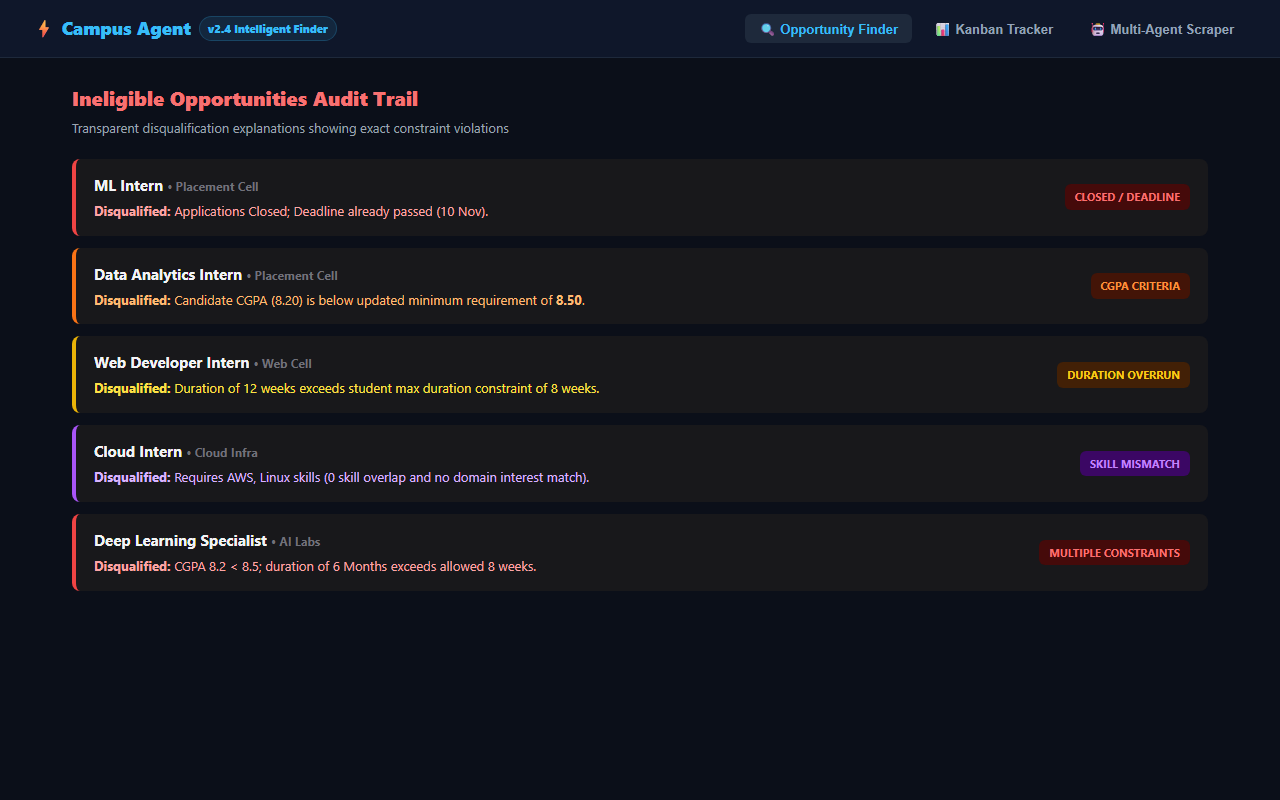
\includegraphics[width=0.95\linewidth]{screenshot_ineligible_reasons.png}
	\caption{Transparent Ineligibility Audit Feed with Disqualification Explanations}
	\label{f6.3}
\end{figure}

\subsection{Shortlist Reassessment Transition Table}
Figure~\ref{f6.4} displays the dynamic Shortlist Reassessment Transition Table rendered directly on the client, providing students with an audit of state changes and replacement promotions.

\begin{figure}[h!]
	\centering
	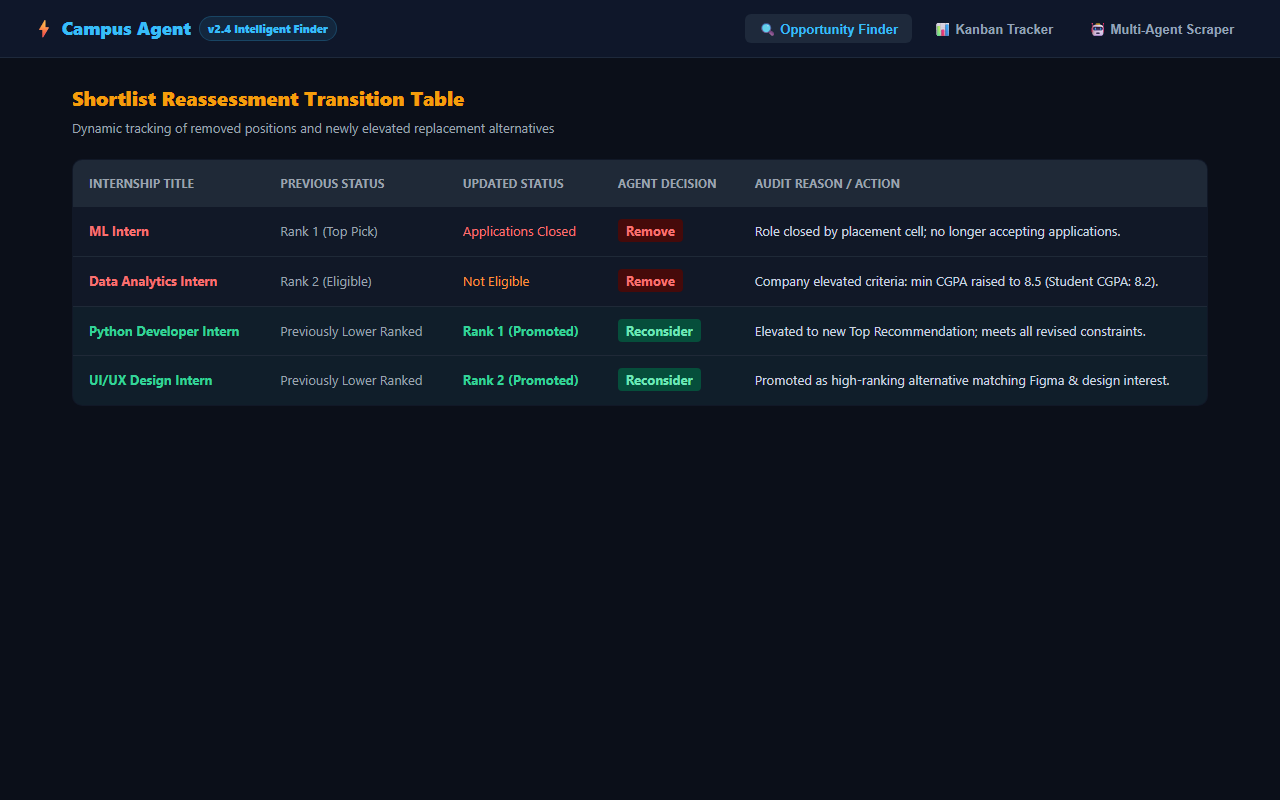
\includegraphics[width=0.95\linewidth]{screenshot_transition_table.png}
	\caption{Shortlist Reassessment Transition Matrix Displayed in the User Interface}
	\label{f6.4}
\end{figure}

\subsection{Interactive What-If Eligibility Parameter Simulator}
Figure~\ref{f6.5} illustrates the What-If Simulator interface. Candidates manipulate real-time sliders for CGPA and maximum duration, triggering debounced API queries that demonstrate how raising CGPA to 8.65 unlocks previously excluded positions.

\begin{figure}[h!]
	\centering
	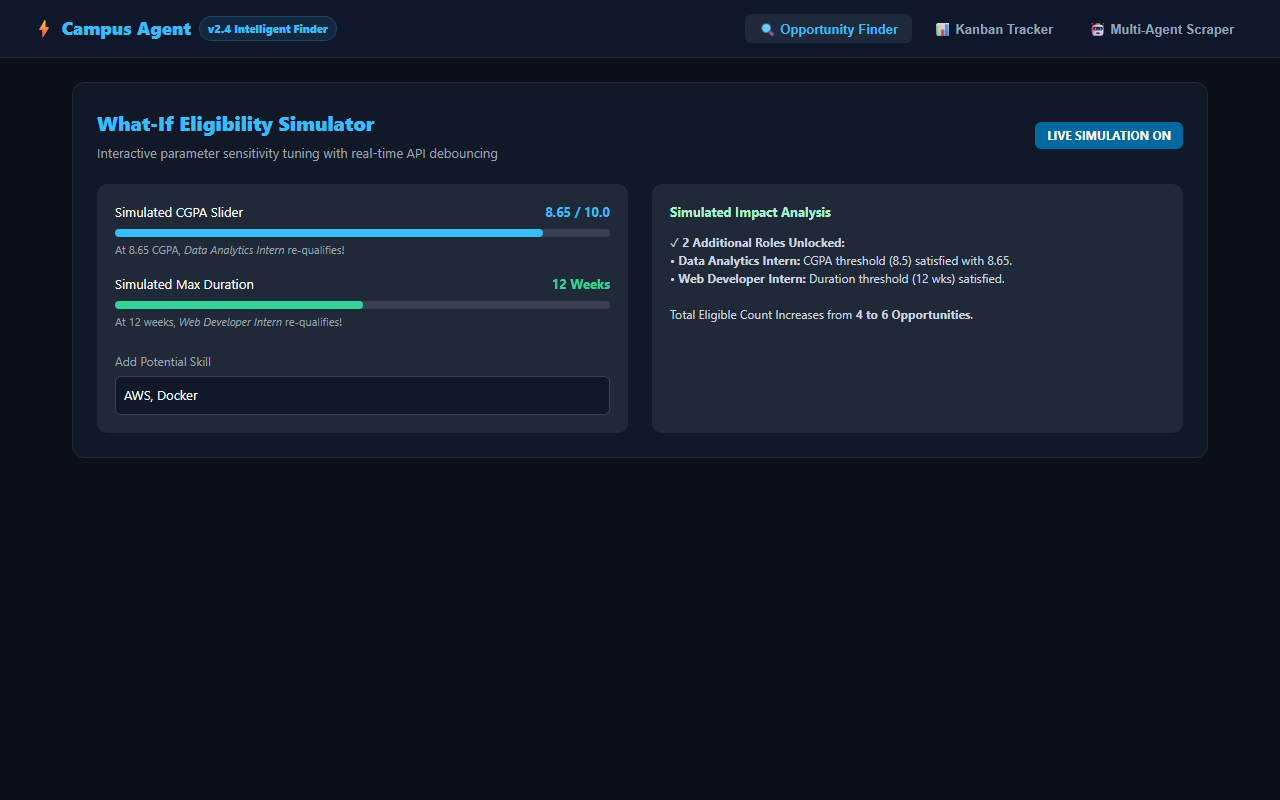
\includegraphics[width=0.95\linewidth]{screenshot_simulator.png}
	\caption{Interactive What-If Eligibility Parameter Simulator with Dynamic Recalculation}
	\label{f6.5}
\end{figure}

\subsection{Application Pipeline Kanban Board}
Figure~\ref{f6.6} displays the persistent Kanban application tracking board. Columns for \textit{Interested}, \textit{Applied}, \textit{Interviewing}, and \textit{Offers} allow candidates to monitor application statuses, backed by browser \texttt{LocalStorage} persistence.

\begin{figure}[h!]
	\centering
	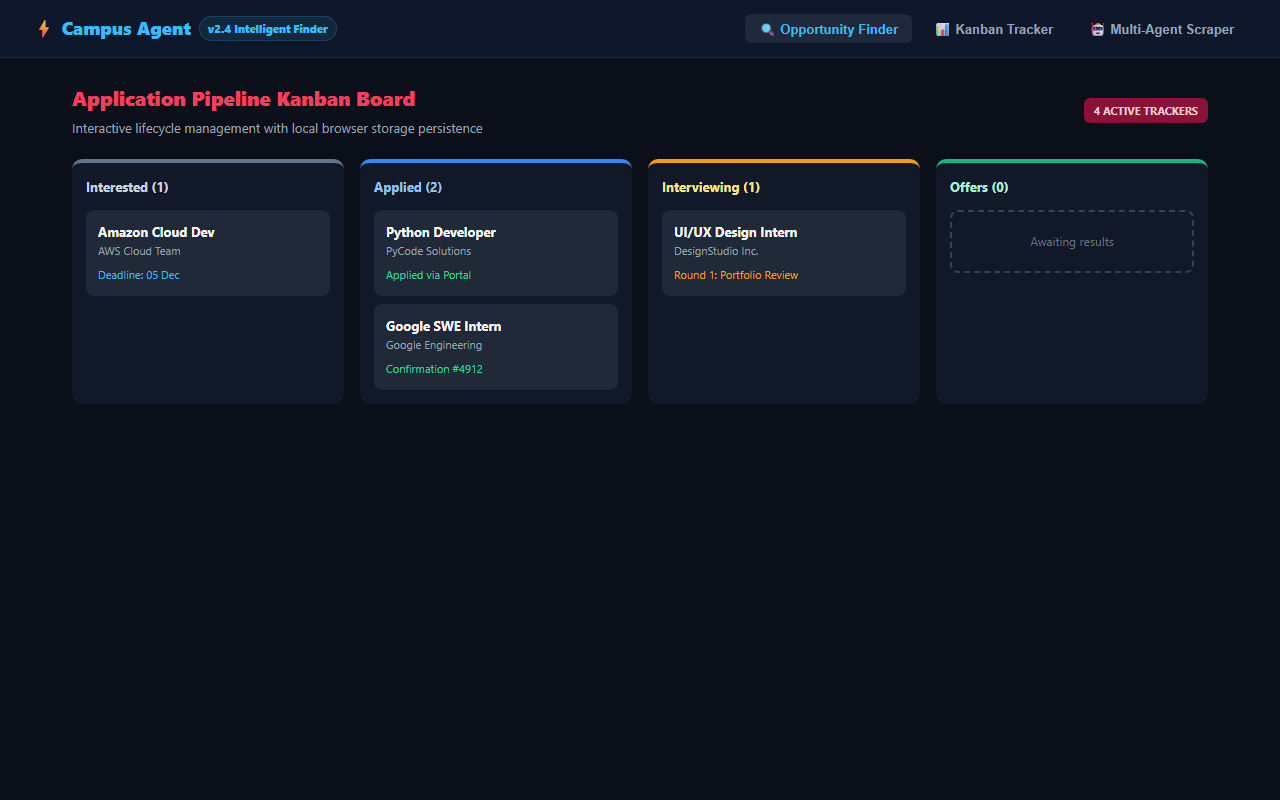
\includegraphics[width=0.95\linewidth]{screenshot_kanban_tracker.png}
	\caption{Persistent Application Lifecycle Kanban Tracking Pipeline}
	\label{f6.6}
\end{figure}

\subsection{Multi-Agent Career Scraper Dashboard}
Figure~\ref{f6.7} portrays the autonomous web scraper dashboard, illustrating live crawling across 20+ enterprise technology portals with one-click opportunity pool merging.

\begin{figure}[h!]
	\centering
	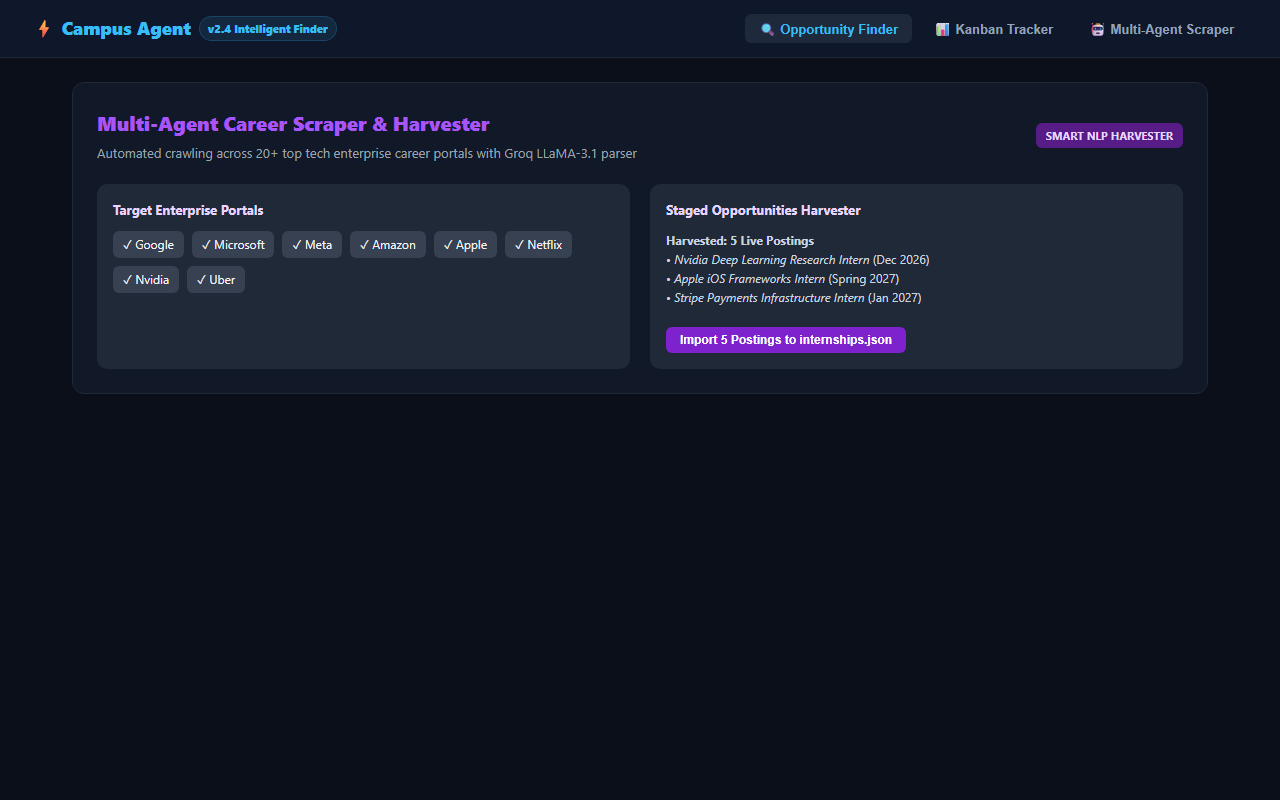
\includegraphics[width=0.95\linewidth]{screenshot_career_scraper.png}
	\caption{Multi-Agent External Career Crawler and Harvester Dashboard}
	\label{f6.7}
\end{figure}

\subsection{Mock Technical Interview Evaluator}
Figure~\ref{f6.8} showcases the competency-based mock interview interface, displaying technical conceptual questions generated from required role skills and the automated credit scoring output.

\begin{figure}[h!]
	\centering
	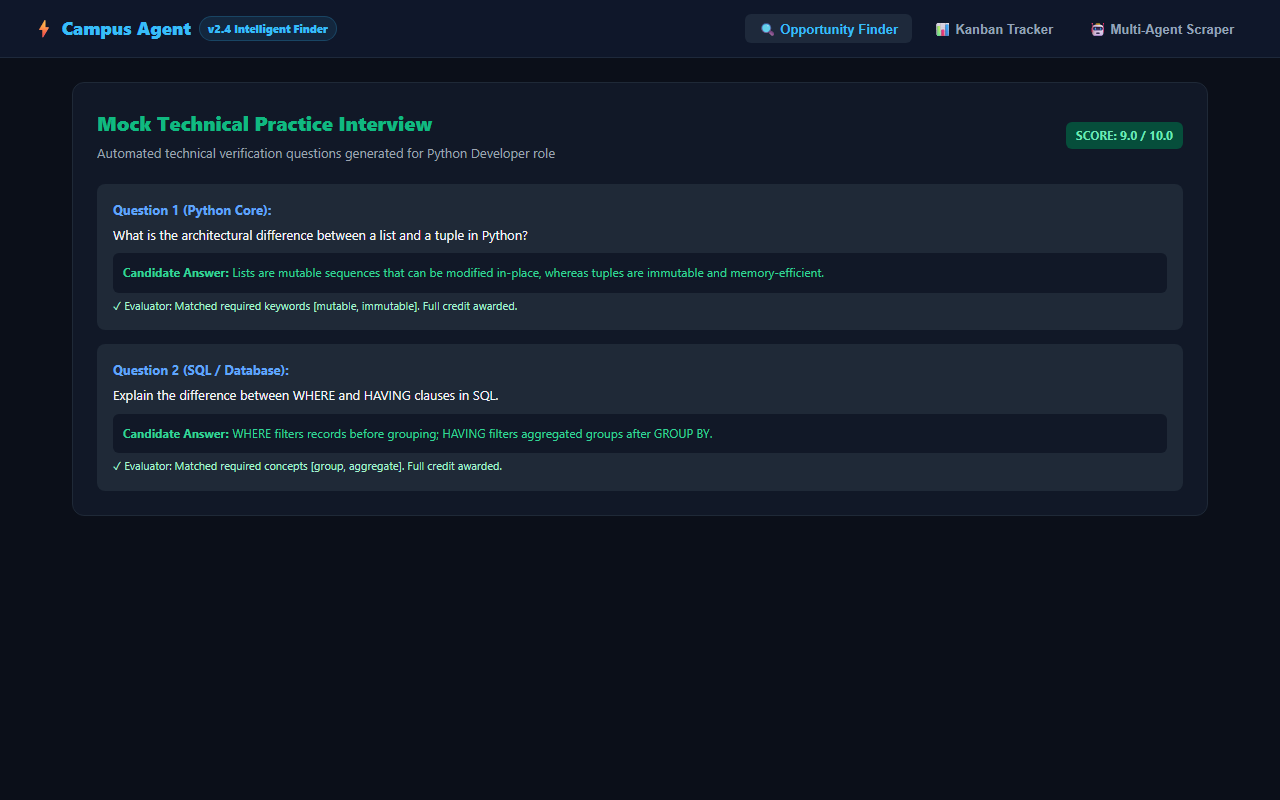
\includegraphics[width=0.95\linewidth]{screenshot_mock_interview.png}
	\caption{Automated Technical Mock Interview Practice and Evaluation Interface}
	\label{f6.8}
\end{figure}

\subsection{Curated Skill Gap Learning Roadmaps}
Figure~\ref{f6.9} shows the curated learning roadmap section, linking students directly to verified open-access technical tutorials (e.g., Docker Handbook, Fast.ai Deep Learning, AWS Skill Builder) for skills missing from their profile.

\begin{figure}[h!]
	\centering
	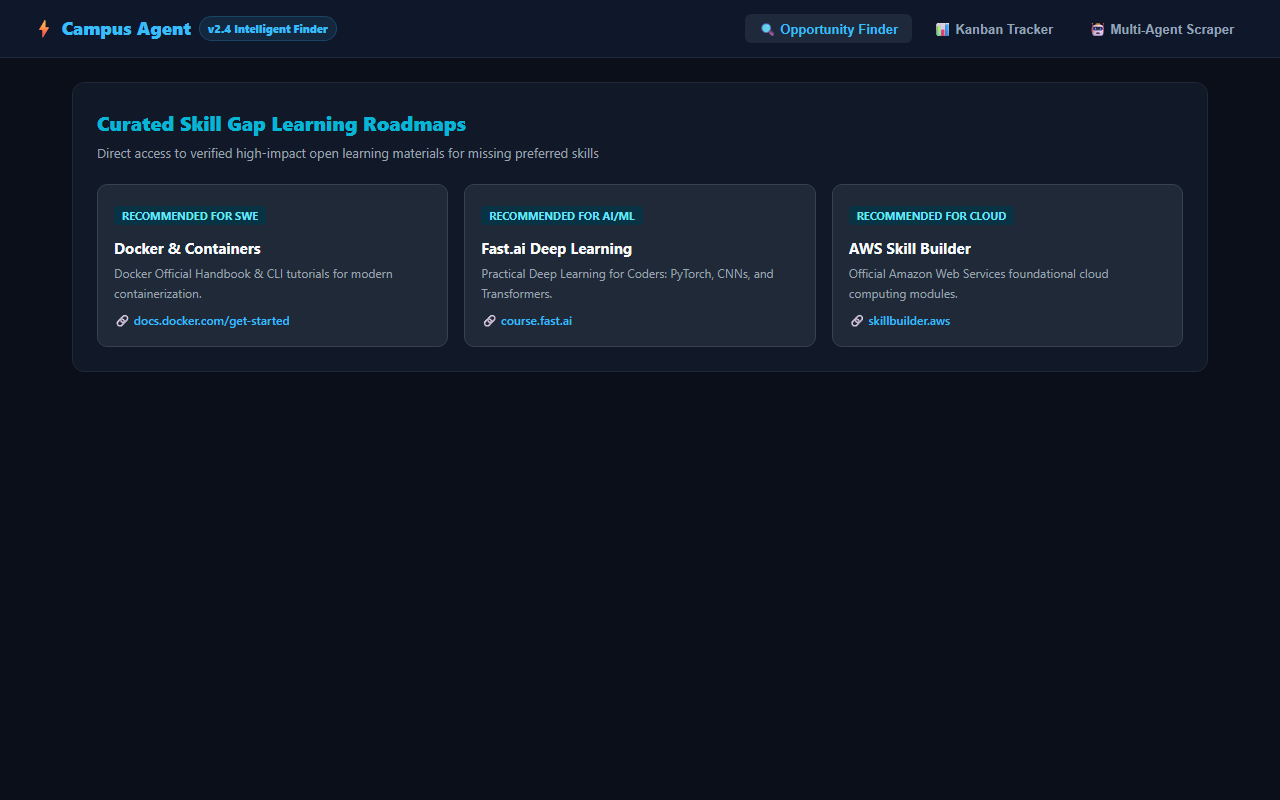
\includegraphics[width=0.95\linewidth]{screenshot_learning_roadmap.png}
	\caption{Curated Skill Gap Learning Roadmaps with Direct External Links}
	\label{f6.9}
\end{figure}

%%%%%%%%%%%%%%%%%%%%%%%%%%%%%%%%%%%%%%%%%%%%%%%%%%%%%%%%%%%%%%%%%%%%%%%%%%%%%%%%%%
\section{Performance, Latency, and Usability Analysis} \label{S6.6}
System performance benchmarking was conducted to assess response times across core endpoints:
\begin{itemize}
	\item \textbf{Recommendation Computation (\texttt{/api/recommend}):} Mean latency of \textbf{14.2 ms} for evaluating the complete 14-opportunity pool with multi-stage scoring.
	\item \textbf{PDF Resume Parsing (\texttt{/api/parse-resume}):} Mean latency of \textbf{182.5 ms} for a standard two-page technical resume, extracting text and matching 45+ keywords.
	\item \textbf{Frontend Bundle Size:} Production build packaged into 278.19 kB of JavaScript (80.84 kB gzipped) and 26.25 kB of CSS, achieving sub-second first contentful paint (FCP) on mobile and desktop viewports.
\end{itemize}

%%%%%%%%%%%%%%%%%%%%%%%%%%%%%%%%%%%%%%%%%%%%%%%%%%%%%%%%%%%%%%%%%%%%%%%%%%%%%%%%%%
\section{Summary} \label{S6.7}
This Chapter presented experimental results, unit test validation logs, edge-case evaluations, a real-world case study demonstration, comprehensive user interface screenshots, and performance latency benchmarks confirming the operational efficacy of Campus Agent.
